\documentclass{article}
\usepackage[utf8]{inputenc}
\usepackage[letterpaper,left=2cm, right=2cm, top=2.5cm, bottom=2.5cm]{geometry}
\usepackage{fancyhdr}
%%%%%%%%%%%%%%%%%%%%%%%%%%%%%%%%%%%%%%%%%%%%%%%%%%%%%%%%%%%%%%
\usepackage{amssymb}
\usepackage{amsmath}
\usepackage{rotating}
\usepackage{graphicx}
\graphicspath{{img/}}
\usepackage{wrapfig}
\usepackage[mathscr]{euscript}
\usepackage[dvipsnames,svgnames,table]{xcolor}
\usepackage{multicol}
\usepackage{multirow}
\usepackage{physics}
\usepackage[version=4]{mhchem}
\usepackage[spanish,es-nodecimaldot,es-tabla]{babel}
\usepackage{parskip}
\usepackage{hyperref}
\usepackage{apacite}
\usepackage{etoolbox}
%%%%%%%%%%%%%%%%%%%%%%%%%%%%%%%%%%%%%%%%%%%%%%%%%%%%%%%%%%%%%%
%\input{definitions}
%\input{qmdef}
\newcommand{\be}{\begin{equation*}}
\newcommand{\ee}{\end{equation*}}
\newcommand{\ble}[1]{\begin{equation} \label{#1}}
\newcommand{\bae}{\begin{eqnarray}}
\newcommand{\eae}{\end{eqnarray}}
\newcommand{\sint}{\sin{\theta}}
\newcommand{\cost}{\cos{\theta}}
\newcommand{\pl}{\left(}
\newcommand{\pr}{\right)}
\newcommand{\kl}{\left[}
\newcommand{\kr}{\right]}
\newcommand{\ii}{\int_{-\infty}^\infty}
\providecommand{\abs}[1]{\lvert#1\rvert}
\providecommand{\norm}[1]{\lVert#1\rVert}
\newcommand{\pa}{\vspace{2mm}}
\definecolor{Grayo}{RGB}{72, 72, 72}
\definecolor{Graya}{RGB}{158, 158, 158}
%%%%%%%%%%%%%%%%%%%%%%%%%%%%%%%%%%%%%%%%%%%%%%%%%%%%%%%%%%%%%%

\begin{document}

\centerline{\Large \textbf{\textcolor{Grayo}{Guía Planeación I}}}
\vspace{2mm}
\centerline{\large \textsc{Christopher López Ruiz}}

\vspace{-10pt}

\begin{center}
\line(1,0){480}
\end{center}

%%%%%%%%%%%%%%%%%%%%%%%%%%%%%%%%%%%%%%%%%%%%%%%%%%%%%
%%%%                                                               Problemas                                                                %%%%
%%%%%%%%%%%%%%%%%%%%%%%%%%%%%%%%%%%%%%%%%%%%%%%%%%%%%

%%%%%%%%%%%%%%%%%%%%%%%%%%%%%%%%%%%%%%%%%%%%%%%%%%%%%

\vspace{3pt}
%%%%%%%%%%%%%%%%%%%%%%%  PROBLEMA 1  %%%%%%%%%%%%%%%%%%%%%%
%%%%%%%%%%%%%%%%%%%%%%%%%%%%%%%%%%%%%%%%%%%%%%%%%%%%%
%

\section*{AP-PA}

\begin{wrapfigure}{l}{0.2\textwidth}
    \centering
    \includegraphics[width=0.2\textwidth]{APPA.pdf}
\end{wrapfigure}

\subsection*{Preinspección}

Visualizar la CT junto a su origen, revisar la orientación e identificar el PTV de interés.

\subsection*{Nuevo Plan}

Se inserta una nueva etapa de tratamiento, posteriormente en esta etapa se inserta un nuevo plan con el PTV de referencia, seleccionar tipo de tratamiento, equipo, posición y energía. 

\textbf{Redondear el isocentro considerando tolerancias de 5 decimales.}

\subsection*{Añadir campos}

Automáticamente se crea un campo con un ángulo de $0^{\circ}$, a partir de este se crea un campo opuesto para poder obtener la disposición de campos de la figura ???.



\vspace{3pt}
%%%%%%%%%%%%%%%%%%%%%%%  PROBLEMA 2 %%%%%%%%%%%%%%%%%%%%%%
%%%%%%%%%%%%%%%%%%%%%%%%%%%%%%%%%%%%%%%%%%%%%%%%%%%%%\vspace{1mm}

\section*{AP-PA/Oblicuos}

\vspace{3pt}
%%%%%%%%%%%%%%%%%%%%%%%  PROBLEMA 3  %%%%%%%%%%%%%%%%%%%%%%
%%%%%%%%%%%%%%%%%%%%%%%%%%%%%%%%%%%%%%%%%%%%%%%%%%%%%

\section*{Holocráneo}

\vspace{3pt}
%%%%%%%%%%%%%%%%%%%%%%%  PROBLEMA 4  %%%%%%%%%%%%%%%%%%%%%%
%%%%%%%%%%%%%%%%%%%%%%%%%%%%%%%%%%%%%%%%%%%%%%%%%%%%%

\section*{Caja}

\vspace{3pt}

%%%%%%%%%%%%%%%%%%%%%%%%%%%%%%%%%%%%%%%%%%%%%%%%%%%
%%%%%%%%%%%%%%%%%%%%%%%  PROBLEMA 5  %%%%%%%%%%%%%%%%%%%%%%
%%%%%%%%%%%%%%%%%%%%%%%%%%%%%%%%%%%%%%%%%%%%%%%%%%%%%

\section*{IMRT}
    
\vspace{3pt}

%%%%%%%%%%%%%%%%%%%%%%%%%%%%%%%%%%%%%%%%%%%%%%%%%%%%%%%%%%%%%%

\begin{center}
\line(1,0){480}
\end{center}

\end{document}

%%%%%%%%%%%%%%%%%%%%%%%%%%%%%%%%%%%%

%\begin{figure}[h]
    %\begin{center}
        %\includegraphics[width=0.5\textwidth]{AT.jpg}
    %\end{center}
%\end{figure}